\documentclass[11pt]{article}

\usepackage[T1]{fontenc}
\usepackage[utf8]{inputenc}
\usepackage{amsmath}
\usepackage{array}
\usepackage{booktabs}
\usepackage{enumitem}
\usepackage{etoolbox}
\usepackage[margin=1in]{geometry}
\usepackage{graphicx}
\usepackage{longtable}
\usepackage{microtype}
\usepackage{nameref}
\usepackage{parskip}
\usepackage{tabularx}
\usepackage[table,dvipsnames]{xcolor}
\usepackage{pagecolor}
\usepackage[numbers]{natbib}
\newtoggle{darkmode}
\togglefalse{darkmode}
\newcommand{\docversion}{Draft}

\newcommand{\applytheme}{
  \iftoggle{darkmode}{
    \definecolor{pagebg}{RGB}{28,30,34}
    \definecolor{textfg}{RGB}{234,236,240}
    \definecolor{linkcolor}{RGB}{122,181,255}
    \definecolor{urlcolor}{RGB}{135,214,190}
    \definecolor{citecolor}{RGB}{245,174,102}
  }{
    \definecolor{pagebg}{RGB}{255,255,255}
    \definecolor{textfg}{RGB}{24,24,24}
    \definecolor{linkcolor}{RGB}{0,68,136}
    \definecolor{urlcolor}{RGB}{0,105,91}
    \definecolor{citecolor}{RGB}{126,63,0}
  }
  \pagecolor{pagebg}
  \makeatletter
  \AtBeginDocument{%
    \color{textfg}%
    \def\ps@plain{%
      \let\@mkboth\@gobbletwo
      \let\@oddhead\@empty
      \let\@evenhead\@empty
      \def\@oddfoot{\reset@font\color{textfg}\hfil\thepage\hfil}%
      \let\@evenfoot\@oddfoot}%
    \pagestyle{plain}%
  }
  \makeatother
}

\newcommand{\term}[1]{\textit{#1}}
\newcommand{\code}[1]{\texttt{#1}}
\newcommand{\consensus}{\term{consensus}}
\newcommand{\policy}{\term{policy}}
\newcommand{\bip}[1]{BIP~#1}
\newcommand{\appendixsection}[1]{%
  \refstepcounter{section}%
  \section*{Appendix \Alph{section}. #1}%
  \addcontentsline{toc}{section}{Appendix \Alph{section}. #1}%
}
\newcolumntype{L}[1]{>{\raggedright\arraybackslash}p{#1}}

\makeatletter
\renewcommand*\l@subsection{\@dottedtocline{2}{1.5em}{3.0em}}
\makeatother

\InputIfFileExists{protocol.ver}{}{}
\applytheme
\usepackage[
  unicode,
  bookmarksnumbered,
  bookmarksopen,
  colorlinks=true,
  linktoc=all,
  linkcolor=linkcolor,
  urlcolor=urlcolor,
  citecolor=citecolor
]{hyperref}

\hypersetup{
  pdftitle={Bitcoin Protocol Specification},
  pdfauthor={Prasad Kumkar, Chainscore Labs, Pune, India},
  pdfsubject={Bitcoin protocol specification},
  pdfkeywords={Bitcoin, protocol, specification, consensus, BIP}
}

\title{Bitcoin Protocol Specification}
\author{Prasad Kumkar\\Chainscore Labs\\Pune, India}
\date{Last updated June 25, 2026}

\begin{document}

\hypersetup{pageanchor=false}
\newgeometry{margin=0in}
\begin{titlepage}
\thispagestyle{empty}
\centering
\vspace*{0.62in}

{\LARGE\bfseries Bitcoin Protocol Specification\par}
\vspace{0.20in}
{\large Prasad Kumkar\par}
\vspace{-0.05in}
{\normalsize prasad@chainscorelabs.com\par}
\vspace{-0.05in}
{\normalsize Pune, INDIA\par}
\vspace{0.13in}
{\small Updated: June 25, 2026\par}

\vspace{0.34in}
\noindent\makebox[\paperwidth][c]{%
\iftoggle{darkmode}
  {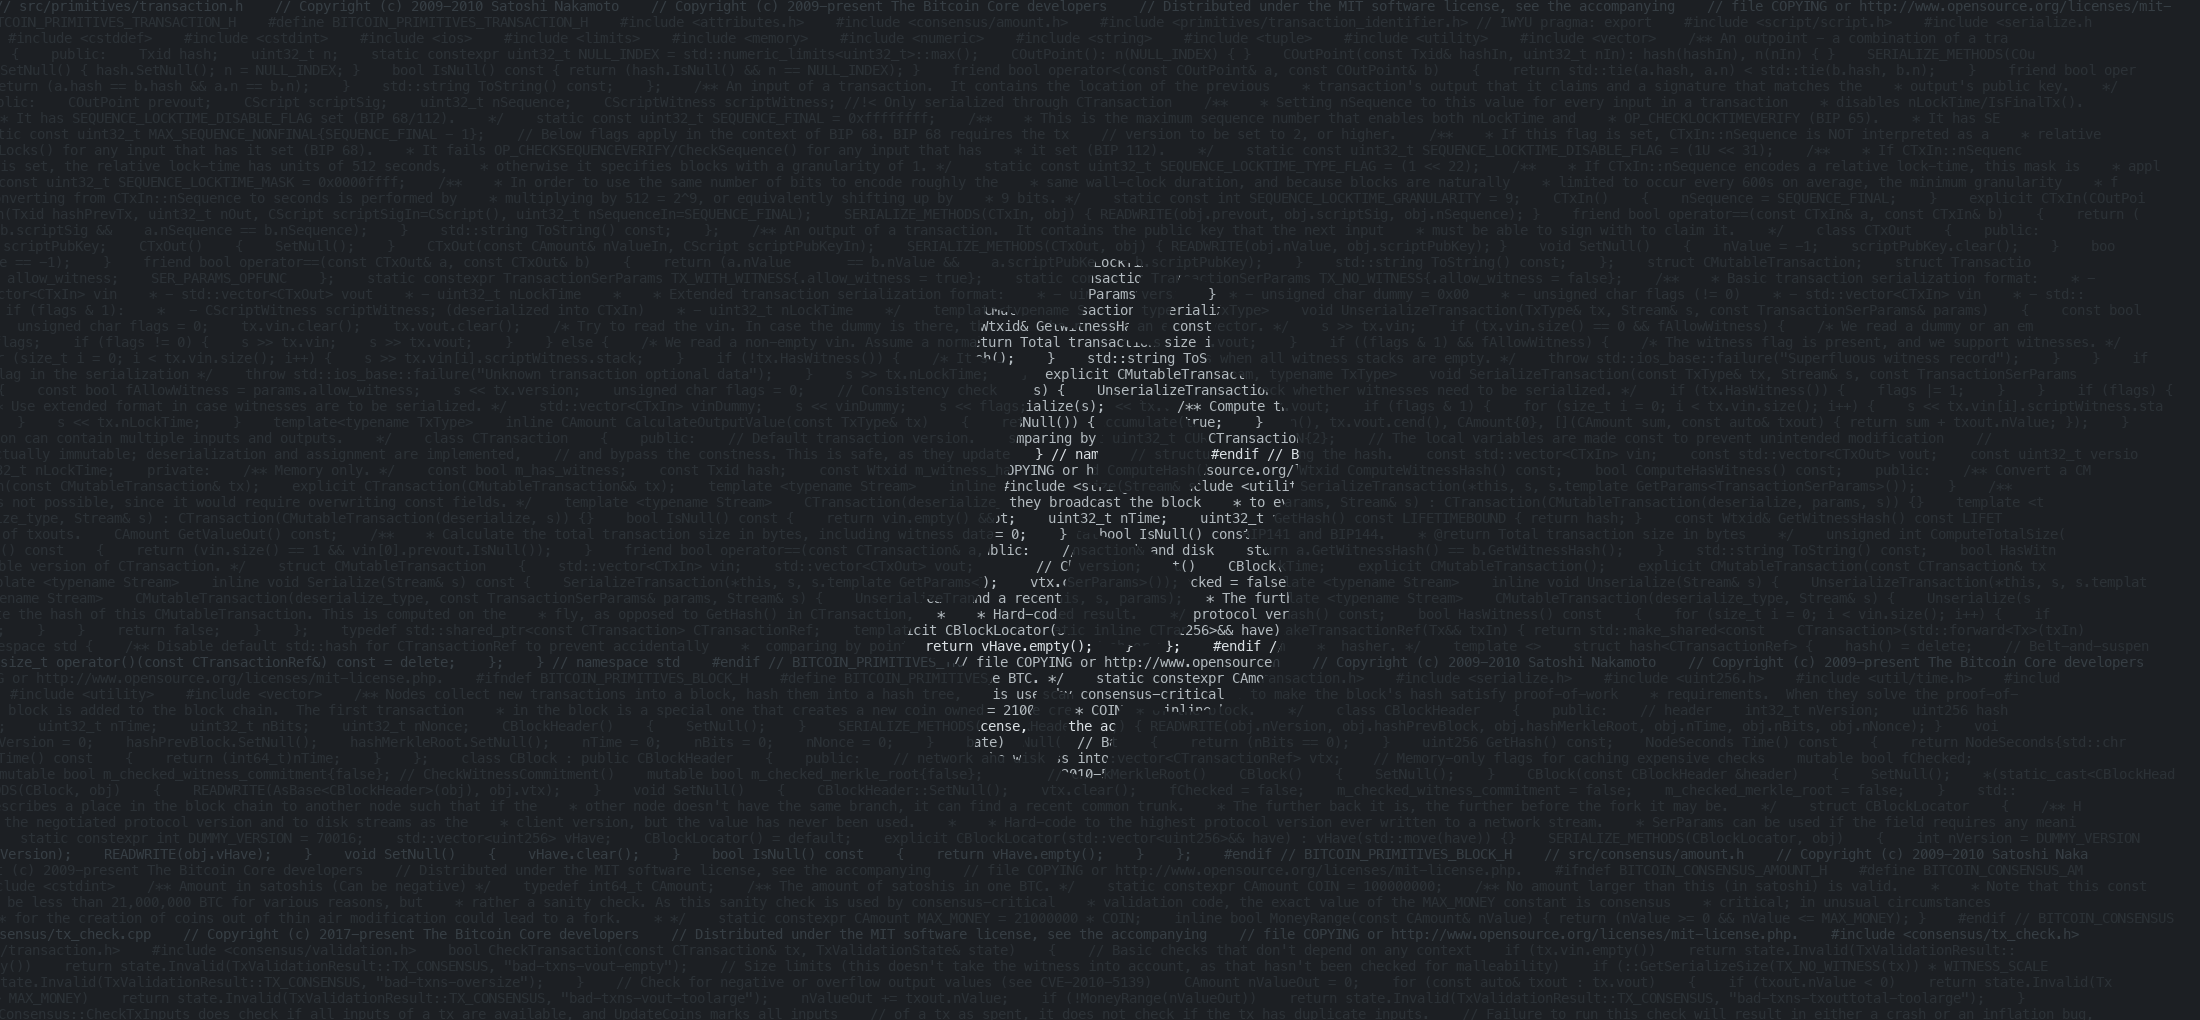
\includegraphics[width=\paperwidth]{assets/bitcoin-core-code-cover-dark.png}}
  {
\includegraphics[width=\paperwidth]{assets/bitcoin-core-code-cover-light.png}}%
}

\vspace{0.46in}
\begin{minipage}{0.72\paperwidth}
\small
\centering
\textbf{Abstract.}

Bitcoin is the peer-to-peer electronic cash protocol and a payment network introduced by Satoshi Nakamoto. This document provides a technical reference and a consolidated knowledge base for the Bitcoin protocol. It is intended to be helpful for Bitcoin-based applications, node clients, and other infrastructure development within the ecosystem. It covers most of the modules implemented by contemporary full nodes: consensus rules, primitive data structures, serialization, peer networking, and relay behavior.

\end{minipage}

\vfill
\vspace*{0.58in}
\end{titlepage}
\restoregeometry
\hypersetup{pageanchor=true}
\iftoggle{darkmode}{\pagestyle{empty}}{}

\tableofcontents
\newpage

\section{Introduction}
\label{sec:introduction}

\subsection{Background}

Bitcoin was introduced by Satoshi Nakamoto as a peer-to-peer electronic cash
system: a network in which payments can be validated by participants directly,
without requiring a financial intermediary to order transactions or prevent
double spending \cite{nakamoto-bitcoin}. Its core design combines digital
signatures, a public append-only history, a proof-of-work timestamp chain, and
local validation by independently operated nodes. Transactions spend previously
created outputs and create new outputs; blocks commit ordered transaction sets;
nodes accept the valid chain with the greatest accumulated proof of work.

The consequence is a protocol whose authority is operational rather than
institutional. No server, committee, or publication grants validity to a
transaction or block. A block is useful only if economically relevant validating
nodes accept it under their consensus rules, and a transaction is final only to
the extent that it remains in the accepted proof-of-work history. This makes
Bitcoin unusually sensitive to precise definitions: serialization, hash
preimages, script evaluation, subsidy, difficulty adjustment, lock-time,
witness commitments, and deployment rules are not merely engineering details.
They are the boundary between a node that follows the same network and a node
that has forked into a different system.

\subsection{Why this specification exists}

Bitcoin does not have a single normative protocol specification in the style of
an Internet RFC. Its design is distributed across the original paper,
Bitcoin Improvement Proposals, Bitcoin Core source code, release notes,
developer documentation, test vectors, and long-running network practice
\cite{bitcoin-bips-repo,bitcoin-core,bitcoin-core-v31,bitcoin-developer-reference}.
That distribution has served Bitcoin well: it keeps proposals reviewable, lets
implementations evolve conservatively, and avoids granting authority to a
document detached from deployed validation behavior. It also leaves developers
with a practical problem. To implement, audit, test, or reason about Bitcoin,
they must assemble one protocol from many artifacts that use different levels
of precision and often mix consensus, policy, wallet behavior, and operational
guidance.

This specification is intended to be the consolidated technical reference for
that protocol. It states Bitcoin as data structures, encodings, identifiers,
state variables, validation predicates, state transitions, and peer messages.
It is not a proposal to change Bitcoin, not a replacement for BIPs, and not an
authority over consensus. Where this document conflicts with economically
relevant node validation, node validation wins. Its purpose is to make the
protocol easier to inspect: one place where the rules needed by independent
implementers, reviewers, researchers, and protocol engineers are expressed
coherently.

\subsection{Related work}

The original Bitcoin paper defines the motivating problem and the high-level
mechanism: timestamped proof of work over a chain of transaction-containing
blocks \cite{nakamoto-bitcoin}. BIPs refine that design by documenting concrete
changes, conventions, and interoperability standards, including consensus soft
forks, peer services, wallet formats, and application-level conventions
\cite{bip-0123,bitcoin-bips-repo}. Bitcoin Core is the dominant full-node
implementation and the principal executable reference for contemporary
validation and relay behavior \cite{bitcoin-core,bitcoin-core-v31}.
Developer references and generated API documentation are valuable guides, but
they are not a complete formal specification of the network protocol
\cite{bitcoin-developer-reference}.

Other cryptocurrency systems have benefited from standalone protocol
specifications. The Zcash protocol specification separates high-level protocol
concepts from concrete encodings and upgrade-specific consensus rules
\cite{zcash-protocol-spec}. Ethereum's Yellow Paper presents Ethereum as a
transaction-based state machine with explicit state-transition functions
\cite{ethereum-yellowpaper}. The JAM graypaper follows the same tradition of a
single coherent formal model for an independently implementable protocol
\cite{graypaper-repo}. This document applies that style to Bitcoin while
respecting Bitcoin's different governance reality: no paper, repository, or
committee has authority to redefine the deployed protocol.

\subsection{Methodology}

The baseline for this draft is Bitcoin Core source, its
implemented-BIPs index, and the BIPs cited throughout this document are treated
as evidence for contemporary full-node behavior
\cite{bitcoin-core-v31}. The specification
separates three classes of behavior:

\begin{enumerate}[leftmargin=*]
  \item Consensus rules: predicates that determine whether blocks and
        transactions can be accepted into the active chain.
  \item Peer and relay rules: network records and local admission behavior used
        by nodes to exchange blocks, transactions, addresses, and negotiation
        state.
  \item Local implementation behavior: storage layout, indexes, caches, RPC
        surfaces, wallet policy, user interface behavior, and performance
        choices that may explain Bitcoin Core but are not themselves protocol
        requirements.
\end{enumerate}

Only the first two classes belong in the main specification. Implementation
details are included only when they expose a protocol boundary or prevent an
ambiguous reading of consensus or peer behavior. This keeps the document useful
as a source-of-truth reference without turning it into a commentary on one code
base.

\section{Notation}
\label{sec:notation}

This section fixes the symbols used across the specification. It defines only
shared notation and reusable primitive relations; concrete record layouts,
script execution, and signature-message construction are defined in their
respective sections.

\subsection{Types and values}

\begin{longtable}{@{}L{0.24\linewidth}L{0.64\linewidth}@{}}
\toprule
Notation & Meaning \\
\midrule
\(\mathbf{Bool}\) & Truth values \(\{\bot,\top\}\). \\
\(\mathbf{Byte}\) & The integers \(\{0,\ldots,255\}\). \\
\(\mathbf{Bytes}\) & Finite byte strings. \\
\(\mathbf{Bytes}[n]\) & Byte strings of exactly \(n\) bytes. \\
\(\mathbf{N}\), \(\mathbf{Z}\) & Nonnegative integers and integers. \\
\(x:T\) & Value \(x\) has type \(T\). \\
\(f:S \to T\) & Total function from \(S\) to \(T\). \\
\(f(x)=\bot\) & \(f\) is undefined, fails, or rejects input \(x\). \\
\bottomrule
\end{longtable}

\subsection{Sequences and records}

\begin{longtable}{@{}L{0.24\linewidth}L{0.64\linewidth}@{}}
\toprule
Notation & Meaning \\
\midrule
\([x_0,\ldots,x_{n-1}]\) & Ordered sequence with zero-based indexing. \\
\(x[i]\) & Element at index \(i\). \\
\(|x|\) & Length of sequence or byte string \(x\). \\
\(x || y\) & Concatenation of sequences or byte strings. \\
\bottomrule
\end{longtable}

Hex strings are written in display order. Sections that describe serialized
fields state whether display order differs from wire order.

Record tables define field order, type, and meaning. Unless explicitly marked
as logical state, a record table gives the order used by \(\mathrm{E}_{T}\).

\subsection{Encoding and byte order}

For a type or record \(T\), \(\mathrm{E}_{T}(x)\) is the canonical byte
encoding of \(x\) as \(T\). The partial inverse
\(\mathrm{E}_{T}^{-1}(b)\) parses bytes \(b\) as \(T\) and is undefined for
non-canonical or invalid encodings. When parsing succeeds,
\(\mathrm{E}_{T}^{-1}(\mathrm{E}_{T}(x))=x\).

\(\mathrm{le}(b)\) is the unsigned little-endian integer represented by byte
string \(b\). Fixed-width integer encodings and CompactSize are defined in
Section~\ref{sec:serialization}.

\subsection{Hashes}

Hash values are protocol bytes. Human display strings often reverse the bytes
of 256-bit hashes.

\[
\begin{aligned}
  \mathrm{H}(b) &= \operatorname{SHA256}(\operatorname{SHA256}(b)),\\
  \operatorname{HASH160}(b) &= \operatorname{RIPEMD160}(\operatorname{SHA256}(b)),\\
  \operatorname{TagHash}_{tag}(b)
    &= \operatorname{SHA256}(\operatorname{SHA256}(tag) ||
       \operatorname{SHA256}(tag) || b).
\end{aligned}
\]

\(\mathrm{H}\) is \code{hash256} in Bitcoin source material. Taproot and
BIP340 Schnorr signatures use \(\operatorname{TagHash}\)
\cite{nakamoto-bitcoin,bip-0340,bip-0341}.

For a nonempty list of 32-byte hashes \(L\), \(\mathrm{MR}(L)\) is the Merkle
root obtained by repeatedly replacing adjacent pairs \((a,b)\) with
\(\mathrm{H}(a||b)\). If a level has odd length, the final hash is duplicated
for that level. \(\mathrm{MR}([])=\bot\).

\subsection{Identifiers}

\[
\begin{aligned}
  txid(tx) &= \mathrm{H}(\mathrm{E}_{0}(tx)),\\
  wtxid(tx) &=
    \begin{cases}
      \mathrm{H}(\mathrm{E}_{w}(tx)), & \text{witness serialization is used},\\
      txid(tx), & \text{otherwise},
    \end{cases}\\
  \mathrm{bh}(h) &= \mathrm{H}(\mathrm{E}_{\mathrm{BlockHeader}}(h)).
\end{aligned}
\]

\subsection{Chain context}

For a chain \(C\), \(C[k]\) is the block at height \(k\), with \(C[0]\) as
genesis. \(\operatorname{height}(B)\) is the height of block \(B\), and
\(\operatorname{tip}(C)=C[|C|-1]\). \(\operatorname{MTP}(C,k)\) is the median
timestamp of \(C[k]\) and its ten nearest ancestors, or all available ancestors
when \(k<10\).

\subsection{Cryptographic relations}

All public-key signature relations use the secp256k1 group.
\(\operatorname{ECDSAVerify}(Q,m,\sigma)\) is true iff ECDSA signature
\(\sigma\) verifies digest \(m\) under public key \(Q\), subject to active script
encoding rules. \(\operatorname{SchnorrVerify}(Q,m,\sigma)\) is the BIP340
verification relation \cite{bip-0066,bip-0340}.

\section{Serialization}
\label{sec:serialization}

Bitcoin protocol objects are byte strings with fixed field order. Unless a
field table states otherwise, \(\mathrm{E}_{T}\) serializes integers in
little-endian byte order, vectors with a CompactSize element count, and byte
vectors with a CompactSize byte length followed by exactly that many bytes.

\subsection{Fixed-width primitives}

\begin{longtable}{@{}L{0.22\linewidth}L{0.18\linewidth}L{0.48\linewidth}@{}}
\toprule
Primitive & Width & Serialization rule \\
\midrule
\code{uint8} / \code{int8} & 1 byte & Byte value as stored. \\
\code{uint16} / \code{int16} & 2 bytes & Least significant byte first. \\
\code{uint32} / \code{int32} & 4 bytes & Least significant byte first. \\
\code{uint64} / \code{int64} & 8 bytes & Least significant byte first. \\
\code{byte[n]} & $n$ bytes & Exactly the given bytes, in index order. \\
\code{bool} & 1 byte & Zero is false; nonzero is true unless a field table restricts the value. \\
\code{uint160} & 20 bytes & 160-bit hash value. \\
\code{uint256} & 32 bytes & 256-bit hash value. Display hex commonly reverses these bytes. \\
\bottomrule
\end{longtable}

Fixed-width integer fields are serialized in little-endian byte order unless a
field table explicitly states otherwise \cite{bitcoin-core-v31}.

\subsection{CompactSize}

Bitcoin transaction and block structures use CompactSize integers to encode
counts and byte-vector lengths. CompactSize is canonical: a decoder rejects a
value encoded with a longer form than necessary.

\begin{longtable}{@{}L{0.24\linewidth}L{0.24\linewidth}L{0.40\linewidth}@{}}
\toprule
Value range & Encoding & Canonicality rule \\
\midrule
$0 \le n < 253$ & one byte: $n$ & First byte is less than 0xfd. \\
$253 \le n \le 0xffff$ & 0xfd followed by \code{uint16} & Decoded value must be at least 253. \\
$2^{16} \le n \le 2^{32}-1$ & 0xfe followed by \code{uint32} & Decoded value must be at least 0x10000. \\
$2^{32} \le n \le 2^{64}-1$ & 0xff followed by \code{uint64} & Decoded value must be at least 0x100000000. \\
\bottomrule
\end{longtable}

A parser rejects non-canonical CompactSize encodings and any decoded count or
length that exceeds the enclosing field's rule.

\subsection{Constructors}

\begin{longtable}{@{}L{0.20\linewidth}L{0.32\linewidth}L{0.36\linewidth}@{}}
\toprule
Constructor & Serialized form & Used for \\
\midrule
\code{vector<T>} & \code{compactSize count || T[0] || ... || T[count-1]} & Transaction inputs, outputs, block transactions, inventory vectors, and payload lists. \\
\code{varbytes} & \code{compactSize length || byte[length]} & Scripts, signatures, public keys, witness items, and variable network fields. \\
\code{string} & \code{compactSize length || byte[length]} & P2P user-agent and payload strings. Character validity is context-specific. \\
\code{witnessStack} & \code{compactSize itemCount || varbytes[0] || ...} & One witness stack for one transaction input. \\
\bottomrule
\end{longtable}

Scripts, signatures, public keys, witness items, and network payload fields
reuse \code{varbytes} in different contexts. Parsing bytes into opcodes,
signatures, keys, or scripts is a later semantic step.

For transactions and blocks, \(\mathrm{E}_{0}(x)\) is the serialization with
witness data stripped, and \(\mathrm{E}_{w}(x)\) is the serialization including
witness data where such data is defined. Define:

\[
  strippedSize(x) = |\mathrm{E}_{0}(x)|,
  \qquad
  totalSize(x) = |\mathrm{E}_{w}(x)|.
\]

The consensus weight formula is:

\[
  weight(x) = 3 \cdot strippedSize(x) + totalSize(x).
\]

For relay and fee accounting, virtual transaction size is the integer ceiling
of weight divided by witness scale:

\[
  vsize(tx) =
  \left\lfloor
  \frac{weight(tx) + \text{\code{WITNESS\_SCALE\_FACTOR}} - 1}
       {\text{\code{WITNESS\_SCALE\_FACTOR}}}
  \right\rfloor.
\]

Block consensus enforces \code{MAX\_BLOCK\_WEIGHT} against \code{weight(block)}
\cite{bip-0141,bitcoin-core-v31}.

\section{Ledger Model}
\label{sec:ledger-model}

Bitcoin validation is modeled as deterministic state transition over a
proof-of-work header graph, available block data, and the active UTXO set. This
section fixes the shared relations used by later sections.

\subsection{State}

A full-validation node's protocol state is:

\[
  S = (C,H,B,U,Q,\Pi)
\]

\begin{longtable}{@{}L{0.14\linewidth}L{0.24\linewidth}L{0.50\linewidth}@{}}
\toprule
Symbol & Type & Meaning \\
\midrule
\(C\) & \code{ActiveChain} & Ordered sequence of connected blocks from genesis to the active tip. \\
\(H\) & \code{HeaderIndex} & Known block-header graph keyed by block hash, including height, predecessor, target, timestamp, and accumulated work. \\
\(B\) & \code{BlockDataSet} & Full block data known to the node, keyed by block hash. \\
\(U\) & \code{UTXOSet} & Map from unspent outpoints to coin records at the active-chain tip. \\
\(Q\) & \code{Mempool} & Locally accepted unconfirmed transactions. This is relay state, not consensus state. \\
\(\Pi\) & \code{PeerSet} & Connected-peer state and negotiated network capabilities. \\
\bottomrule
\end{longtable}

Consensus validation reads \(C,H,B,U\) and mutates only \(C,H,B,U\). Mempool
and peer transitions read consensus state but do not define block validity.

\subsection{Coins}

The UTXO set maps outpoints to coins:

\[
  U[(txid,n)] = (value, scriptPubKey, height, coinbase).
\]

\begin{longtable}{@{}L{0.22\linewidth}L{0.24\linewidth}L{0.42\linewidth}@{}}
\toprule
Coin field & Type & Meaning \\
\midrule
\code{value} & \code{Amount} & Output amount in satoshis. Consensus-valid values are in the money range. \\
\code{scriptPubKey} & \code{Script} & Locking script committed by the creating transaction output. \\
\code{height} & \code{uint32} & Active-chain height of the creating transaction. \\
\code{coinbase} & \code{bool} & True iff the creating transaction is the block coinbase. \\
\bottomrule
\end{longtable}

\subsection{Rule context}

Let \(N\) be the selected network parameter set. For candidate height \(h\),
candidate block time \(t\), and active chain \(C\), define:

\[
  R = \operatorname{Rules}(N,C,h,t).
\]

\(R\) is the set of consensus rules active for the candidate object. It includes
network constants, buried activation heights, versionbits state, timestamp
rules, and script flags. Later sections use \(R\) rather than restating whether
P2SH, BIP34, strict DER, locktime, sequence locks, SegWit, Taproot, Tapscript,
or network-specific timewarp mitigations are active.

\subsection{Validity classes}

\begin{longtable}{@{}L{0.24\linewidth}L{0.64\linewidth}@{}}
\toprule
Class & Meaning \\
\midrule
\(\operatorname{DecodeValid}_{T}(b)\) & \(\mathrm{E}_{T}^{-1}(b)\) succeeds and consumes a canonical encoding of type \(T\). \\
\(\operatorname{FormValid}(x)\) & Object \(x\) is internally well-formed independent of chain state. \\
\(\operatorname{ContextValid}_{R}(x,C)\) & Object \(x\) satisfies height, time, and active-rule predicates under \(R\). \\
\(\operatorname{StateValid}_{R}(x,U)\) & Object \(x\) is valid against the current spendable coin set. \\
\(\operatorname{RelayValid}_{P}(x,Q,U)\) & Object \(x\) is accepted by local relay policy. This is not a consensus predicate. \\
\bottomrule
\end{longtable}

\subsection{Transition relations}

For a non-coinbase transaction, the transaction transition is:

\[
  \operatorname{ApplyTx}(R,U,tx) =
  \begin{cases}
    U', & \text{if } tx \text{ is valid against } U \text{ under } R,\\
    \bot, & \text{otherwise.}
  \end{cases}
\]

For a block \(B_h\) at height \(h\), block connection is:

\[
  \operatorname{ConnectBlock}(R,(C,U),B_h) =
  \begin{cases}
    (C',U'), & \text{if every block and transaction predicate succeeds,}\\
    \bot, & \text{otherwise.}
  \end{cases}
\]

Header acceptance, block-data acceptance, chain selection, and reorganization
are the consensus transitions defined in Section~\ref{sec:consensus}. Mempool
admission is the local transition defined in Section~\ref{sec:mempool}.

\subsection{Invariants}

Every accepted active-chain transition preserves:

\begin{longtable}{@{}L{0.24\linewidth}L{0.64\linewidth}@{}}
\toprule
Invariant & Statement \\
\midrule
Determinism & For fixed \(N,C,U,B_h\), successful connection produces a unique \(C',U'\). \\
Outpoint uniqueness & At any active tip, each outpoint appears at most once in \(U\). \\
No double spend & A connected transaction consumes each input outpoint at most once, and a connected block consumes each live outpoint at most once. \\
Conservation & A non-coinbase transaction cannot create value: \(\sum outputs(tx) \le \sum spent(tx)\). \\
Issuance bound & For each connected block, \(\sum outputs(coinbase) \le subsidy(h)+\sum fees(B_h)\). \\
Work selection & The active chain is selected from valid candidates by greatest accumulated work. \\
\bottomrule
\end{longtable}

\section{Transactions}
\label{sec:transactions}

A Bitcoin transaction consumes previously created outputs and creates new
outputs. Consensus validation distinguishes the serialized transaction bytes,
the identifiers derived from those bytes, and the contextual checks that depend
on the UTXO set and block height.

\subsection{Identifier and amount primitives}

\begin{longtable}{@{}L{0.22\linewidth}L{0.24\linewidth}L{0.42\linewidth}@{}}
\toprule
Type & Encoding & Meaning \\
\midrule
\code{Txid} & \code{uint256} & \(txid(tx)\), as defined in Section~\ref{sec:notation}. \\
\code{Wtxid} & \code{uint256} & \(wtxid(tx)\), as defined in Section~\ref{sec:notation}. \\
\code{OutPoint} & \code{Txid || uint32} & Reference to one transaction output by transaction identifier and output index. \\
\code{Amount} & \code{int64} & Satoshis. Consensus-valid output amounts satisfy $0 \le value \le$ \code{MAX\_MONEY}. \\
\bottomrule
\end{longtable}

\subsection{Transaction records}

\begin{longtable}{@{}L{0.18\linewidth}L{0.22\linewidth}L{0.22\linewidth}L{0.28\linewidth}@{}}
\toprule
\multicolumn{4}{@{}l}{\textbf{\code{TxOut}}} \\
\midrule
Field & Type & Encoding & Meaning \\
\midrule
\code{value} & \code{Amount} & \code{int64} & Output value in satoshis. \\
\code{scriptPubKey} & \code{Script} & \code{varbytes} & Locking script. \\
\bottomrule
\end{longtable}

\begin{longtable}{@{}L{0.18\linewidth}L{0.22\linewidth}L{0.22\linewidth}L{0.28\linewidth}@{}}
\toprule
\multicolumn{4}{@{}l}{\textbf{\code{TxIn}}} \\
\midrule
Field & Type & Encoding & Meaning \\
\midrule
\code{previousOutput} & \code{OutPoint} & 36 bytes & Output spent by this input, or the null outpoint for coinbase. \\
\code{scriptSig} & \code{Script} & \code{varbytes} & Unlocking script or coinbase data. \\
\code{sequence} & \code{uint32} & 4 little-endian bytes & Finality, replacement, and relative-lock field. \\
\bottomrule
\end{longtable}

\begin{longtable}{@{}L{0.18\linewidth}L{0.22\linewidth}L{0.22\linewidth}L{0.28\linewidth}@{}}
\toprule
\multicolumn{4}{@{}l}{\textbf{\code{Transaction}}} \\
\midrule
Field & Type & Encoding & Meaning \\
\midrule
\code{version} & \code{int32} & 4 little-endian bytes & Transaction version. Versions 1 and 2 are standard by default relay policy; consensus accepts the integer subject to contextual rules. \\
\code{inputs} & \code{vector<TxIn>} & CompactSize count, then inputs & Spent outputs or coinbase input. \\
\code{outputs} & \code{vector<TxOut>} & CompactSize count, then outputs & Created outputs. \\
\code{witnesses} & \code{vector<Witness>} & witness serialization only & One witness stack per input when witness serialization is used. \\
\code{lockTime} & \code{uint32} & 4 little-endian bytes & Absolute height or time lock. \\
\bottomrule
\end{longtable}

\code{Witness} is \code{vector<varbytes>}. It is present only in witness
serialization and has exactly one stack per input.

\subsection{Legacy serialization}

\(\mathrm{E}_{0}(tx)\), the legacy transaction serialization, is:

\[
  version || inputs || outputs || lockTime.
\]

\begin{longtable}{@{}L{0.22\linewidth}L{0.24\linewidth}L{0.42\linewidth}@{}}
\toprule
Part & Encoding & Meaning \\
\midrule
\code{version} & \code{int32} & Transaction version. \\
\code{inputCount} & \code{compactSize} & Number of inputs. \\
\code{inputs} & \code{TxIn[inputCount]} & Serialized inputs in order. \\
\code{outputCount} & \code{compactSize} & Number of outputs. \\
\code{outputs} & \code{TxOut[outputCount]} & Serialized outputs in order. \\
\code{lockTime} & \code{uint32} & Absolute lock field. \\
\bottomrule
\end{longtable}

\subsection{Witness serialization}

\(\mathrm{E}_{w}(tx)\), the witness transaction serialization, is:

\[
  version || marker || flag || inputs || outputs || witnesses || lockTime.
\]

\begin{longtable}{@{}L{0.22\linewidth}L{0.24\linewidth}L{0.42\linewidth}@{}}
\toprule
Part & Encoding & Meaning \\
\midrule
\code{marker} & \code{0x00} & Distinguishes witness serialization from legacy serialization. \\
\code{flag} & \code{0x01} & Indicates witness data follows. Other nonzero flag bits are invalid. \\
\code{witnesses} & \code{Witness[inputCount]} & One witness stack per input. \\
\bottomrule
\end{longtable}

The witness form is valid only when at least one witness stack is nonempty. A
transaction with no witness data uses legacy serialization for both \code{Txid}
and \code{Wtxid} \cite{bip-0141,bip-0144}.

\subsection{Transaction identifiers}

\begin{longtable}{@{}L{0.22\linewidth}L{0.58\linewidth}@{}}
\toprule
Identifier & Definition \\
\midrule
\code{txid(tx)} & Defined in Section~\ref{sec:notation}. \\
\code{wtxid(tx)} & Defined in Section~\ref{sec:notation}. \\
\code{GenTxid} & Pair of identifier kind and hash used by relay to distinguish txid and wtxid announcements. \\
\bottomrule
\end{longtable}

\subsection{Context-free validity}

A transaction is context-free valid only if:

\begin{enumerate}[leftmargin=*]
  \item it has at least one input and at least one output;
  \item its stripped size satisfies
        $strippedSize(tx) \cdot
        \text{\code{WITNESS\_SCALE\_FACTOR}}
        \le \text{\code{MAX\_BLOCK\_WEIGHT}}$;
  \item every output value is in range;
  \item the sum of output values is in range;
  \item no two inputs reference the same previous output;
  \item if it is coinbase, it has exactly one input whose previous output is
        the null outpoint and whose \code{scriptSig} length is between
        \code{COINBASE\_SCRIPTSIG\_MIN} and
        \code{COINBASE\_SCRIPTSIG\_MAX} bytes; and
  \item if it is not coinbase, no input uses the null outpoint.
\end{enumerate}

Context-free validity does not prove the inputs exist or signatures are valid;
those checks require the UTXO set and rule context
\cite{bitcoin-core-v31}.

\subsection{Coinbase transaction}

A coinbase transaction has exactly one input whose previous output is the null
outpoint defined by \code{NULL\_TXID} and \code{NULL\_INDEX}. Its input does not
spend a UTXO. Its outputs create the block subsidy and collect fees, subject to
the coinbase amount rule during block connection.

Coinbase-created outputs require \code{COINBASE\_MATURITY} confirmations before
they may be spent.

\subsection{Value conservation}

For a non-coinbase transaction:

\[
  fee(tx) = \sum value(spentInputs(tx)) - \sum value(outputs(tx)).
\]

The transaction is invalid if any referenced input is absent, any spent coin is
immature coinbase, any output is outside the money range, the output sum is
outside the money range, or \code{fee(tx)} is negative
\cite{bitcoin-core-v31}.

\subsection{Locktime and sequence}

\code{lockTime} values below \code{LOCKTIME\_THRESHOLD} are block heights;
values at or above that threshold are Unix times. For a candidate block at
height \(h\) with rule context \(R\) and locktime cutoff \(t\), define the
selected lock boundary:

\[
\ell(tx,h,t)=
\begin{cases}
h,
  & tx.\text{\code{lockTime}} < \text{\code{LOCKTIME\_THRESHOLD}},\\
t,
  & tx.\text{\code{lockTime}} \ge \text{\code{LOCKTIME\_THRESHOLD}},
\end{cases}
\]

\[
\begin{aligned}
\operatorname{AbsFinal}(tx,h,t) \Longleftrightarrow\;&
tx.\text{\code{lockTime}}=0 \vee
tx.\text{\code{lockTime}} < \ell(tx,h,t) \vee {}\\
&\forall i:\ tx.\text{\code{inputs}}[i].\text{\code{sequence}}
  = \text{\code{SEQUENCE\_FINAL}}.
\end{aligned}
\]

If \(R\) includes BIP113, \(t=\operatorname{MTP}(C,h-1)\); otherwise \(t\) is
the candidate block timestamp.

If \(R\) includes BIP68, relative locks apply only to version-2-or-higher
transactions and only to inputs whose \code{sequence} does not set
\code{SEQUENCE\_LOCKTIME\_DISABLE\_FLAG}. For validation view \(V\), define
\(\operatorname{SeqFinal}(tx,C,V,h)\) as follows. If
\(tx.\text{\code{version}} < 2\), it is true. Otherwise, for each applicable
input \(i\), let \(s_i\) be its sequence value, \(v_i=s_i \mathbin{\&}
\text{\code{SEQUENCE\_LOCKTIME\_MASK}}\), and \(c_i\) be the height of
the coin spent by input \(i\) in \(V\). Height locks require:

\[
  h > c_i + v_i - 1.
\]

When \(s_i\) sets \code{SEQUENCE\_LOCKTIME\_TYPE\_FLAG}, the input is time
locked instead. Let \(\tau_i=\operatorname{MTP}(C,c_i-1)\). Time locks require:

\[
  \operatorname{MTP}(C,h-1) >
  \tau_i + v_i \cdot \text{\code{SEQUENCE\_LOCKTIME\_GRANULARITY}} - 1.
\]

The transaction satisfies relative locks iff every applicable input satisfies
its selected height or time constraint; disabled inputs impose no constraint.
If \(R\) does not include BIP68, \(\operatorname{SeqFinal}\) is true
\cite{bip-0068,bip-0112,bip-0113,bitcoin-core-v31}.

\subsection{Signature hashes}

Signature validation signs a digest derived from the transaction, input index,
spent output, hash type, and active script version. Legacy, SegWit v0, and
Taproot/Tapscript spend paths use different digest algorithms, specified in
Section~\ref{sec:script}. These digests are consensus-critical because the
signature checks validate exactly those bytes.

\section{Script Execution}
\label{sec:script}

For each non-coinbase input \(i\), spend authorization is the predicate:

\[
  \operatorname{Authorize}_{R}(tx,i,coin,u,H) \in \{\top,\bot\},
\]

where \(u=(scriptSig,witness)\) is the unlocking data, \(coin\) is the spent
UTXO, \(R\) is the active rule context, and \(H\) is the candidate height and
median-time context. Authorization chooses a spend form, constructs a script
machine state, and evaluates the committed program.

\subsection{Spend forms}

\begin{longtable}{@{}L{0.24\linewidth}L{0.64\linewidth}@{}}
\toprule
Form & Required relation \\
\midrule
Legacy & \(\operatorname{Eval}_{R}(scriptSig,\mathrm{BASE})\) then \(\operatorname{Eval}_{R}(scriptPubKey,\mathrm{BASE})\); witness empty; final stack top is true. \\
P2SH & \(R\) includes P2SH; \code{scriptSig} is push-only; final pushed item is \code{redeemScript}; \(\operatorname{HASH160}(redeemScript)\) matches; \(\operatorname{Eval}_{R}(redeemScript,\mathrm{BASE})\) succeeds on the pushed stack. \\
Witness v0 key hash & Native witness program length 20; \code{scriptSig} empty unless P2SH-wrapped; witness stack is \((signature,pubkey)\); \(\operatorname{HASH160}(pubkey)\) matches; ECDSA verifies \(M_{\mathrm{wit0}}\). \\
Witness v0 script hash & Native witness program length 32; final witness item is \code{witnessScript}; \(\operatorname{SHA256}(witnessScript)\) matches; \(\operatorname{Eval}_{R}(witnessScript,\mathrm{WITNESS\_V0})\) succeeds on the remaining witness stack. \\
Taproot key path & \(R\) includes Taproot; witness stack, after optional annex removal, contains one Schnorr signature; BIP340 verifies \(M_{\mathrm{tr}}\) under the output key. \\
Taproot script path & Control block commits a tapleaf to the output key. Leaf version \code{0xc0} evaluates as Tapscript; unknown leaf versions succeed after commitment validation. \\
Unknown witness version & A syntactically valid witness program with no assigned meaning succeeds without execution. \\
\bottomrule
\end{longtable}

Native witness spends require empty \code{scriptSig}; P2SH-wrapped witness
spends require \code{scriptSig} to push exactly the witness program
\cite{bip-0016,bip-0141,bip-0143,bip-0340,bip-0341,bip-0342}.

\subsection{Machine state}

Script evaluation is a deterministic transition over:

\[
  X=(tx,i,coin,script,pc,S,A,C,R,\sigma,k,\alpha,\beta).
\]

\begin{longtable}{@{}L{0.18\linewidth}L{0.70\linewidth}@{}}
\toprule
Field & Meaning \\
\midrule
\code{script}, \code{pc} & Program bytes and instruction cursor. \\
\(S,A,C\) & Main stack, altstack, and conditional-execution stack. \\
\(R,\sigma\) & Active rule context and signature version: \(\mathrm{BASE}\), \(\mathrm{WITNESS\_V0}\), or \(\mathrm{TAPSCRIPT}\). \\
\(k\) & Last executed code-separator position for signature-message construction. \\
\(\alpha\) & Taproot annex, if present. \\
\(\beta\) & Tapscript validation-weight budget. \\
\bottomrule
\end{longtable}

Legacy and witness-v0 execution enforce the script limits named in
Appendix~\ref{app:constants}. Tapscript removes the script-size and
per-script-opcode limits, keeps the stack-item and stack-size limits, and sets:

\[
  \beta =
  \text{\code{TAPSCRIPT\_SIGOPS\_BUDGET\_BASE}}+
  \operatorname{serializedWitnessSize}(input).
\]

Each executed signature opcode with a nonempty signature subtracts
\code{TAPSCRIPT\_SIGOPS\_COST}; negative \(\beta\) fails.

\subsection{Evaluation}

\[
  \operatorname{Eval}_{R}(script,\sigma,S_0)=
  \begin{cases}
    \top, & \text{execution halts successfully with required final stack,}\\
    \bot, & \text{parsing, execution, resource, or final-stack validation fails.}
  \end{cases}
\]

If \(\sigma=\mathrm{TAPSCRIPT}\), the script is scanned for any
\code{OP\_SUCCESSx} index before ordinary execution; encountering one succeeds.
Otherwise, instructions are decoded left to right and \(\operatorname{Step}\)
is applied while all entries of \(C\) are true. Non-control opcodes in inactive
branches do not mutate \(S\), but parse-stage failures and Tapscript
\code{OP\_SUCCESSx} detection still apply.

Successful termination requires an empty \(C\). Legacy and witness-v0 require a
nonempty \(S\) whose top element casts to true. Tapscript requires exactly one
stack element, and that element must cast to true.

\subsection{Primitive relations}

\begin{longtable}{@{}L{0.28\linewidth}L{0.60\linewidth}@{}}
\toprule
Relation & Definition \\
\midrule
\(\operatorname{CastToBool}(x)\) & False iff \(x\) is empty, zero, or negative zero; true otherwise. \\
\(\operatorname{Num}(x,n,min)\) & Signed-magnitude little-endian integer from byte vector \(x\), length at most \(n\); if \(min\), nonzero encodings must be minimal. \\
\(\operatorname{MinimalPush}(op,x)\) & True iff \(op\) is the shortest permitted push form for \(x\). \\
\(\operatorname{LockTime}(X,n)\) & Units match \code{tx.lockTime}, \(n\le tx.lockTime\), and the input sequence is nonfinal. \\
\(\operatorname{Sequence}(X,n)\) & BIP68 is active in \(R\), disable/type bits permit comparison, and the input sequence satisfies \(n\). \\
\(\operatorname{CheckSig}(X,sig,key,h)\) & Empty signatures return false. Legacy and witness-v0 use ECDSA over secp256k1; Taproot and Tapscript use BIP340 Schnorr. Tapscript key size 0 fails, size 32 verifies, and other nonzero key sizes are unknown key types that pass current consensus. \\
\bottomrule
\end{longtable}

\subsection{Signature messages}

Signature checks verify exactly one digest:

\[
\begin{aligned}
  M_{\mathrm{legacy}} &= \operatorname{SigMsg}_{\mathrm{legacy}}(tx,i,k,h),\\
  M_{\mathrm{wit0}} &= \operatorname{SigMsg}_{\mathrm{wit0}}(tx,i,coin,k,h),\\
  M_{\mathrm{tr}} &= \operatorname{SigMsg}_{\mathrm{tr}}(tx,i,coin,\alpha,k,h).
\end{aligned}
\]

Hash type bytes are \code{0x00} \code{DEFAULT} for Taproot,
\code{0x01} \code{ALL}, \code{0x02} \code{NONE}, \code{0x03}
\code{SINGLE}, and \code{0x80} \code{ANYONECANPAY} ORed with non-default
forms. \code{ALL}, \code{NONE}, and \code{SINGLE} select the output commitment
set; \code{ANYONECANPAY} restricts input commitment to the signed input.
Legacy out-of-range \code{SINGLE} signs \code{uint256::ONE}; Taproot
out-of-range \code{SINGLE} fails \cite{bip-0143,bip-0341,bip-0342}.

\subsection{Opcode classes}

Effects use \code{(before -- after)} for stack transitions, with the rightmost
item at the top of \(S\). Every opcode index is covered by exactly one row
below.

\begin{longtable}{@{}L{0.14\linewidth}L{0.34\linewidth}L{0.40\linewidth}@{}}
\toprule
Index & Opcode & Effect \\
\midrule
\code{0} & \code{OP\_0 / OP\_FALSE} & Push empty vector. \\
\code{1..75} & \code{OP\_PUSHBYTES\_n} & Push the next \(n\) script bytes. \\
\code{76} & \code{OP\_PUSHDATA1} & Next \code{uint8} gives pushed byte length. \\
\code{77} & \code{OP\_PUSHDATA2} & Next little-endian \code{uint16} gives pushed byte length. \\
\code{78} & \code{OP\_PUSHDATA4} & Next little-endian \code{uint32} gives pushed byte length. \\
\code{79} & \code{OP\_1NEGATE} & Push \(-1\). \\
\code{81..96} & \code{OP\_1..OP\_16} & Push integer \(1..16\). \\
\bottomrule
\end{longtable}

\begin{longtable}{@{}L{0.14\linewidth}L{0.34\linewidth}L{0.40\linewidth}@{}}
\toprule
Index & Opcode & Effect \\
\midrule
\code{97} & \code{OP\_NOP} & No effect. \\
\code{99} & \code{OP\_IF} & \code{(v --)}; push \(\operatorname{CastToBool}(v)\) to \(C\). \\
\code{100} & \code{OP\_NOTIF} & \code{(v --)}; push negated condition to \(C\). \\
\code{101} & \code{OP\_VERIF} & Fail. \\
\code{102} & \code{OP\_VERNOTIF} & Fail. \\
\code{103} & \code{OP\_ELSE} & Toggle top of \(C\); unmatched \code{ELSE} fails. \\
\code{104} & \code{OP\_ENDIF} & Pop top of \(C\); unmatched \code{ENDIF} fails. \\
\code{105} & \code{OP\_VERIFY} & \code{(v --)} if true; otherwise fail. \\
\code{106} & \code{OP\_RETURN} & Fail. \\
\bottomrule
\end{longtable}

\begin{longtable}{@{}L{0.14\linewidth}L{0.34\linewidth}L{0.40\linewidth}@{}}
\toprule
Index & Opcode & Effect \\
\midrule
\code{107} & \code{OP\_TOALTSTACK} & Move top of \(S\) to \(A\). \\
\code{108} & \code{OP\_FROMALTSTACK} & Move top of \(A\) to \(S\). \\
\code{109..114} & \code{OP\_2DROP..OP\_2SWAP} & Fixed stack rearrangements; fail on underflow. \\
\code{115} & \code{OP\_IFDUP} & Duplicate top item iff it casts true. \\
\code{116} & \code{OP\_DEPTH} & Push stack depth. \\
\code{117..125} & \code{OP\_DROP..OP\_TUCK} & Fixed stack rearrangements; fail on underflow. \\
\code{130} & \code{OP\_SIZE} & \code{(x -- x len(x))}. \\
\bottomrule
\end{longtable}

\begin{longtable}{@{}L{0.14\linewidth}L{0.34\linewidth}L{0.40\linewidth}@{}}
\toprule
Index & Opcode & Effect \\
\midrule
\code{135} & \code{OP\_EQUAL} & Byte-vector equality. \\
\code{136} & \code{OP\_EQUALVERIFY} & Equality followed by \code{VERIFY}. \\
\code{139..148} & \code{OP\_1ADD..OP\_SUB} & Unary or binary arithmetic over \(\operatorname{Num}(x,4,min)\). \\
\code{154..165} & \code{OP\_BOOLAND..OP\_WITHIN} & Boolean and numeric comparisons over \(\operatorname{Num}(x,4,min)\). \\
\bottomrule
\end{longtable}

\begin{longtable}{@{}L{0.14\linewidth}L{0.34\linewidth}L{0.40\linewidth}@{}}
\toprule
Index & Opcode & Effect \\
\midrule
\code{166} & \code{OP\_RIPEMD160} & \code{(x -- RIPEMD160(x))}. \\
\code{167} & \code{OP\_SHA1} & \code{(x -- SHA1(x))}. \\
\code{168} & \code{OP\_SHA256} & \code{(x -- SHA256(x))}. \\
\code{169} & \code{OP\_HASH160} & \code{(x -- HASH160(x))}. \\
\code{170} & \code{OP\_HASH256} & \code{(x -- H(x))}. \\
\code{171} & \code{OP\_CODESEPARATOR} & Set \(k\) to this opcode position. \\
\code{172} & \code{OP\_CHECKSIG} & \code{(sig key -- ok)} using \(\operatorname{CheckSig}\). \\
\code{173} & \code{OP\_CHECKSIGVERIFY} & \code{CHECKSIG} followed by \code{VERIFY}. \\
\code{174} & \code{OP\_CHECKMULTISIG} & \code{(dummy sig[m] m key[n] n -- ok)}; enforces historical dummy rule when active; disabled in Tapscript. \\
\code{175} & \code{OP\_CHECKMULTISIGVERIFY} & \code{CHECKMULTISIG} followed by \code{VERIFY}; disabled in Tapscript. \\
\code{186} & \code{OP\_CHECKSIGADD} & Tapscript only: \code{(sig n key -- n+ok)}. \\
\bottomrule
\end{longtable}

\begin{longtable}{@{}L{0.14\linewidth}L{0.34\linewidth}L{0.40\linewidth}@{}}
\toprule
Index & Opcode & Effect \\
\midrule
\code{176} & \code{OP\_NOP1} & No effect. \\
\code{177} & \code{OP\_CHECKLOCKTIMEVERIFY / OP\_NOP2} & If active in \(R\), require \(\operatorname{LockTime}(X,n)\); otherwise no effect. \\
\code{178} & \code{OP\_CHECKSEQUENCEVERIFY / OP\_NOP3} & If active in \(R\), require \(\operatorname{Sequence}(X,n)\); otherwise no effect. \\
\code{179..185} & \code{OP\_NOP4..OP\_NOP10} & No effect unless redefined by active soft-fork rules. \\
\bottomrule
\end{longtable}

\begin{longtable}{@{}L{0.14\linewidth}L{0.34\linewidth}L{0.40\linewidth}@{}}
\toprule
Index & Opcode & Effect \\
\midrule
\code{80} & \code{OP\_RESERVED / OP\_SUCCESS80} & Reserved failure if executed outside Tapscript; Tapscript success. \\
\code{98} & \code{OP\_VER / OP\_SUCCESS98} & Reserved failure if executed outside Tapscript; Tapscript success. \\
\code{126..129} & \code{OP\_CAT..OP\_RIGHT / OP\_SUCCESSx} & Disabled failure outside Tapscript; Tapscript success. \\
\code{131..134} & \code{OP\_INVERT..OP\_XOR / OP\_SUCCESSx} & Disabled failure outside Tapscript; Tapscript success. \\
\code{137..138} & \code{OP\_RESERVED1..OP\_RESERVED2 / OP\_SUCCESSx} & Reserved failure if executed outside Tapscript; Tapscript success. \\
\code{141..142} & \code{OP\_2MUL..OP\_2DIV / OP\_SUCCESSx} & Disabled failure outside Tapscript; Tapscript success. \\
\code{149..153} & \code{OP\_MUL..OP\_RSHIFT / OP\_SUCCESSx} & Disabled failure outside Tapscript; Tapscript success. \\
\code{187..254} & \code{OP\_SUCCESS187..OP\_SUCCESS254} & Tapscript success; invalid outside Tapscript. \\
\code{255} & \code{OP\_INVALIDOPCODE} & Fail. \\
\bottomrule
\end{longtable}

Consensus script behavior is defined by the active P2SH, DER, locktime,
sequence, NULLDUMMY, SegWit, Taproot, and Tapscript rules
\cite{bip-0065,bip-0066,bip-0068,bip-0112,bip-0113,bip-0147,bip-0341,bip-0342,bitcoin-core-v31}.

\section{Blocks}
\label{sec:blocks}

A block is a header plus an ordered transaction vector. The header commits to
the previous block header, transaction Merkle root, timestamp, target encoding,
and nonce. The transaction vector begins with exactly one coinbase transaction.

\subsection{Block header}

A serialized \code{BlockHeader} is exactly 80 bytes in the field order shown:

\begin{longtable}{@{}L{0.18\linewidth}L{0.18\linewidth}L{0.22\linewidth}L{0.32\linewidth}@{}}
\toprule
\multicolumn{4}{@{}l}{\textbf{\code{BlockHeader}}} \\
\midrule
Field & Type & Encoding & Meaning \\
\midrule
\code{version} & \code{int32} & 4 little-endian bytes & Block version. Version bits use the high-bit pattern defined by \bip{9}. \\
{\small\code{previous}\newline\code{BlockHash}} & \code{uint256} & 32 bytes & Double-SHA256 hash of the previous block header in protocol byte order. \\
\code{merkleRoot} & \code{uint256} & 32 bytes & Merkle root of transaction identifiers. Witness data is committed separately. \\
\code{time} & \code{uint32} & 4 little-endian bytes & Miner-supplied Unix timestamp. \\
\code{bits} & \code{uint32} & 4 little-endian bytes & Compact proof-of-work target encoding. \\
\code{nonce} & \code{uint32} & 4 little-endian bytes & Nonce varied during proof-of-work search. \\
\bottomrule
\end{longtable}

For a block \(B\), \(\mathrm{bh}(B)=\mathrm{bh}(B.\text{\code{header}})\).

\subsection{Block record}

\begin{longtable}{@{}L{0.18\linewidth}L{0.20\linewidth}L{0.22\linewidth}L{0.30\linewidth}@{}}
\toprule
\multicolumn{4}{@{}l}{\textbf{\code{Block}}} \\
\midrule
Field & Type & Encoding & Meaning \\
\midrule
\code{header} & \code{BlockHeader} & 80 bytes & Serialized block header. \\
\code{txCount} & \code{compactSize} & CompactSize & Number of serialized transactions. \\
\code{transactions} & {\small\code{vector<}\newline\code{Transaction>}} & transaction encodings in order & First transaction must be coinbase; all later transactions must not be coinbase. \\
\bottomrule
\end{longtable}

When witness data is present, block serialization includes each transaction's
witness serialization for relay and block-weight computation. The transaction
identifier Merkle root continues to use \code{txid}, not \code{wtxid}.

\subsection{Merkle root}

For a block transaction vector \([tx_0,\ldots,tx_{n-1}]\), define:

\[
  L = [txid(tx_0), txid(tx_1), \ldots, txid(tx_{n-1})].
\]

A block commits to \(\mathrm{MR}(L)\). A block with empty \(L\) is invalid.

During root computation, a node rejects the duplicated-subtree mutation case:
if two identical hashes are paired at a level before an odd-last duplication
step, the block is invalid as mutated
\cite{bitcoin-core-v31}.

\subsection{Coinbase transaction}

The first transaction in each block is the coinbase transaction. It is the only
transaction permitted to have a null prevout. No other transaction in a block
may be coinbase. The coinbase creates the block subsidy and collects transaction
fees; its total output value must not exceed subsidy plus fees when the block is
connected.

\(\operatorname{Rules}(N,C,h,t)\) determines whether the candidate height must
be serialized at the beginning of the coinbase \code{scriptSig}
\cite{bip-0034,bitcoin-core-v31}.

\subsection{Witness commitment}

If \(R=\operatorname{Rules}(N,C,h,t)\) includes SegWit and any transaction has
witness data, the coinbase must commit to the witness Merkle root. The witness
tree leaves are:

\[
  W = [0^{256}, wtxid(tx_1), \ldots, wtxid(tx_{n-1})].
\]

The coinbase input witness contains a 32-byte reserved value \(r\). The
witness commitment is:

\[
  wc = \mathrm{H}(\mathrm{MR}(W) || r).
\]

The commitment appears in a coinbase output whose script begins with the
SegWit commitment header. If multiple outputs match, the highest-index matching
output is used \cite{bip-0141}.

\subsection{Context-free block checks}

\begin{longtable}{@{}L{0.28\linewidth}L{0.60\linewidth}@{}}
\toprule
Check & Rule \\
\midrule
Transaction count & The block contains at least one transaction. \\
Transaction count weight & \code{txCount * WITNESS\_SCALE\_FACTOR <= MAX\_BLOCK\_WEIGHT}. \\
Coinbase position & Transaction zero is coinbase; no later transaction is coinbase. \\
Merkle root & Header \code{merkleRoot} equals \(\mathrm{MR}(L)\) and is not mutated. \\
Stripped size & \code{strippedSize(block) * WITNESS\_SCALE\_FACTOR <= MAX\_BLOCK\_WEIGHT}. \\
Transaction validity & Every transaction passes context-free transaction checks. \\
Legacy sigops & \code{legacySigOps(block) * WITNESS\_SCALE\_FACTOR <= MAX\_BLOCK\_SIGOPS\_COST}. \\
\bottomrule
\end{longtable}

\subsection{Contextual block checks}

For a candidate block at height \(h\) extending chain \(C\), the previous block
is \(C[h-1]\), and \(R=\operatorname{Rules}(N,C,h,\code{time})\).

\begin{longtable}{@{}L{0.28\linewidth}L{0.60\linewidth}@{}}
\toprule
Check & Rule \\
\midrule
Previous header & The previous header exists and is valid for extension. \\
Median time & \code{time} is greater than \(\operatorname{MTP}(C,h-1)\). \\
Future time & A node does not accept the block while \code{time} is more than \code{MAX\_FUTURE\_BLOCK\_TIME} after the node's current clock time; this is temporary future status, not permanent consensus invalidity. \\
BIP94 timewarp & On networks enforcing BIP94, the first block of each difficulty-adjustment interval except genesis must have \code{time >= previous.time - BIP94\_TIMEWARP\_GRACE}. \\
Difficulty & \code{bits} encodes the target required for the height and network. \\
Finality & All transactions satisfy \(\operatorname{AbsFinal}(tx,h,t)\), where \(t=\operatorname{MTP}(C,h-1)\) if \(R\) includes BIP113 and the candidate block time otherwise. \\
Coinbase height & If \(R\) includes BIP34, the block commits to the correct height in the coinbase. \\
Witness commitment & If \(R\) includes SegWit and the block has witness data, the block contains the correct coinbase witness commitment. \\
Weight & Block weight is at most \code{MAX\_BLOCK\_WEIGHT}. \\
\bottomrule
\end{longtable}

The timestamp checks above follow the active validation predicates for median
time past, future-time acceptance, and BIP94 timewarp mitigation
\cite{bitcoin-core-v31,bip-0094}.

\section{Proof of Work and Chain Selection}
\label{sec:pow}

Bitcoin blocks commit to proof of work through the block header hash. A block is
valid only if its header hash satisfies the target encoded by the header's
\code{nBits} field.

\subsection{Target encoding}

The \code{nBits} field is a 32-bit compact target. For compact value \(c\), let:

\[
  e = c \gg 24,\qquad
  m = c \mathbin{\&} 0x007fffff,\qquad
  s = c \mathbin{\&} 0x00800000.
\]

The decoded target \(\mathrm{C}^{-1}(c)\) is:

\[
\mathrm{C}^{-1}(c) =
\begin{cases}
  m \gg 8(3-e), & e \le 3,\\
  m \ll 8(e-3), & e > 3.
\end{cases}
\]

The sign bit is inherited from an older multiple-precision integer format and is
not permitted for proof-of-work targets. A decoded target is invalid if any of
the following conditions holds:

\begin{itemize}[leftmargin=*]
  \item \(s\) is set and \(m \ne 0\);
  \item \(\mathrm{C}^{-1}(c)=0\);
  \item decoding overflows 256 bits, which occurs when \(m \ne 0\) and either
        \(e > 34\), or \(m > 0xff\) and \(e > 33\), or \(m > 0xffff\) and \(e > 32\);
  \item \(\mathrm{C}^{-1}(c)\) is greater than the network's proof-of-work limit.
\end{itemize}

This compact-target decoding matches contemporary Bitcoin Core consensus
validation \cite{bitcoin-core-v31}.

The compact encoding \(\mathrm{C}(T)\) of target \(T\) is computed as follows. Let
\code{size = ceil(bitLength(T) / 8)}. If \code{size <= 3}, set
\code{word = T << 8(3 - size)}; otherwise set
\code{word = T >> 8(size - 3)}. If \code{word} has bit \code{0x00800000} set,
right-shift \code{word} by 8 and increment \code{size}. Then:

\[
  \mathrm{C}(T) = (size \ll 24) \mathbin{|} (word \mathbin{\&} 0x007fffff).
\]

Consensus proof-of-work targets are nonnegative, so the sign bit is not set in
valid block targets.

\subsection{Proof-of-work check}

For header \(h\), let:

\[
  T_h = \mathrm{C}^{-1}(h.\text{\code{bits}}),\qquad p_h = \mathrm{le}(\mathrm{bh}(h)).
\]

A candidate block satisfies proof of work iff \(T_h\) is a valid target and:

\[
  p_h \le T_h.
\]

A node rejects the block header if target decoding fails or if the hash integer
is greater than the target. The network-specific proof-of-work limit is part of
the chain parameters, not a value inferred from the genesis block
\cite{bitcoin-core-v31}.

\subsection{Difficulty adjustment}

Mainnet difficulty adjusts over fixed-height intervals. Test networks can have
different adjustment behavior. Network-specific exceptions must be cited from
chain parameter sources rather than inferred from mainnet behavior.

For mainnet:
\[
  \text{\code{DIFFICULTY\_ADJUSTMENT\_INTERVAL}} =
  \frac{\text{\code{TARGET\_TIMESPAN}}}{\text{\code{TARGET\_SPACING}}}.
\]
A candidate block's \code{nBits} must equal the value returned by the network's
difficulty-adjustment function for the previous block and candidate timestamp
\cite{bitcoin-core-v31}.

For networks without the minimum-difficulty exception, the algorithm is:

\begin{enumerate}[leftmargin=*]
  \item If the candidate height is not an exact difficulty-adjustment interval,
        return the previous block's \code{nBits}.
  \item Otherwise, identify the first block in the previous adjustment period.
        For mainnet this is the ancestor
        \code{DIFFICULTY\_ADJUSTMENT\_INTERVAL - 1} blocks before
        \code{previous}.
  \item Compute
        $\Delta = time(previous) - time(first)$.
  \item Clamp $\Delta$ to the range
        \[
          \frac{\text{\code{TARGET\_TIMESPAN}}}{\text{\code{MAX\_RETARGET\_FACTOR}}}
          \le \Delta \le
          \text{\code{TARGET\_TIMESPAN}} \cdot
          \text{\code{MAX\_RETARGET\_FACTOR}}.
        \]
  \item Decode the previous period's base target. On testnet4-like networks with
        BIP94 enforcement, the base target is taken from the first block of the
        period; otherwise it is taken from the previous block.
  \item Set:
        \[
          T' =
          \frac{baseTarget \cdot \Delta}{\text{\code{TARGET\_TIMESPAN}}}.
        \]
  \item If $T'$ exceeds the network proof-of-work limit, use the proof-of-work
        limit.
  \item Return \(\mathrm{C}(T')\).
\end{enumerate}

On no-retarget networks, the function returns the previous block's
\code{nBits}. On networks that allow special minimum-difficulty blocks, the
function may return the proof-of-work limit when the candidate timestamp is more
than \(2 \cdot \text{\code{TARGET\_SPACING}}\) after the previous block;
otherwise it searches backward for the most recent non-special difficulty in the
current adjustment period \cite{bitcoin-core-v31}.

\subsection{Accumulated work}

Nodes compare competing valid chains by accumulated work rather than by block
count. This follows the proof-of-work security model described in the Bitcoin
whitepaper \cite{nakamoto-bitcoin}.

For each accepted header, the node adds the work implied by that header's target
to the predecessor's accumulated work. Headers and blocks with invalid proof of
work are rejected before they can contribute to active-chain selection.

For a valid compact target, Bitcoin Core computes the work represented by a
header as:

\[
  work(c) =
  \left\lfloor \frac{2^{256}-\mathrm{C}^{-1}(c)-1}{\mathrm{C}^{-1}(c)+1} \right\rfloor + 1.
\]

This is algebraically equivalent to \(\lfloor 2^{256}/(\mathrm{C}^{-1}(c)+1) \rfloor\) while
avoiding construction of the unrepresentable integer $2^{256}$ in a 256-bit
integer type \cite{bitcoin-core-v31}. The active chain is selected from
valid candidates by greatest accumulated work, not by height.

\section{Consensus Validation}
\label{sec:consensus}

Consensus validation determines whether a node may accept a chain history as
valid. It instantiates the transition relations from
Section~\ref{sec:ledger-model} for headers, block data, active-chain
connection, and reorganization.

\subsection{Validation relation}

Let \(N\) be the network parameter set. For candidate block \(b\), candidate
height \(h\), candidate block time \(t\), active chain \(C\), and UTXO set
\(U\), let \(R=\operatorname{Rules}(N,C,h,t)\). A successful connection
produces:

\[
  (C, U) \xrightarrow{b} (C', U')
\]

where \(C'\) extends or reorganizes \(C\) to include \(b\), and \(U'\) is the UTXO set
obtained after applying every transaction in the connected branch. If any
consensus check fails, the active pair \((C,U)\) is unchanged.

\subsection{Header acceptance}

A header is accepted into the header graph only if all conditions below hold.
Header acceptance does not imply that block transaction data is known or valid.

\begin{longtable}{@{}L{0.28\linewidth}L{0.60\linewidth}@{}}
\toprule
Condition & Required rule \\
\midrule
Uniqueness & If \(\mathrm{bh}(h)\) is already known, the existing header state is reused. \\
Previous header & Every non-genesis header references a known previous header. \\
Proof of work & \(\mathrm{le}(\mathrm{bh}(h)) \le \mathrm{C}^{-1}(h.\text{\code{bits}})\). \\
Target & \(\mathrm{C}^{-1}(h.\text{\code{bits}})\) is valid for the height, network, and difficulty-adjustment interval. \\
Timestamp & The header time is greater than the median timestamp of the previous block and up to ten ancestors. A header whose time is more than \code{MAX\_FUTURE\_BLOCK\_TIME} after the node's current clock time is future-dated and not eligible for active validation until time advances. \\
BIP94 timewarp & On networks enforcing BIP94, a difficulty-adjustment block other than genesis has time at least \code{previous.time - BIP94\_TIMEWARP\_GRACE}. \\
Rule context & \(R\) permits the candidate height, time, version field, and network-specific activation state. \\
Invalid ancestry & A header descending from a known-invalid header is not eligible for best-chain selection. \\
\bottomrule
\end{longtable}

For each accepted header, the node records height, predecessor,
\(\mathrm{C}^{-1}(h.\text{\code{bits}})\), \(\mathrm{bh}(h)\), and accumulated
work. Accumulated work is the sum of the work represented by each header from
genesis through that header.

\subsection{Block-data acceptance}

Full block data is accepted only after the corresponding header is accepted.
The following checks are performed before block data can become a candidate for
active-chain connection:

\begin{longtable}{@{}L{0.26\linewidth}L{0.62\linewidth}@{}}
\toprule
Check & Required rule \\
\midrule
Block form & The block has at least one transaction, satisfies the stripped-size, transaction-count, and weight limits in Section~\ref{sec:blocks}, and the first transaction is the only coinbase transaction. \\
Merkle root & Header \code{merkleRoot} equals \(\mathrm{MR}(L)\) for the block's txid leaves, and the mutated-root condition is rejected. \\
Transaction form & Every transaction passes context-free transaction checks. \\
Legacy sigops limit & \code{legacySigOps(block) * WITNESS\_SCALE\_FACTOR <= MAX\_BLOCK\_SIGOPS\_COST} before P2SH and witness sigops are counted during connection. \\
Contextual finality & Every transaction satisfies \(\operatorname{AbsFinal}\) for the candidate block height and locktime cutoff. \\
Coinbase height & If \(R\) includes BIP34, the coinbase script begins with the candidate height. \\
Witness commitment & If \(R\) includes SegWit and the block has witness data, the coinbase witness commitment is present and correct. \\
Weight & The block weight is at most \code{MAX\_BLOCK\_WEIGHT}. \\
\bottomrule
\end{longtable}

\subsection{Best-chain selection}

Among branches whose headers are valid and whose required block data is
available, the selected branch is the valid branch with greatest accumulated
work. A candidate branch is not eligible while any block on the path from the
active fork to the candidate tip is missing block data or is known invalid.

\begin{enumerate}[leftmargin=*]
  \item Choose the highest-work eligible candidate tip.
  \item Find the fork point with the current active chain.
  \item Disconnect active-chain blocks back to the fork.
  \item Connect candidate-branch blocks forward in height order.
  \item If a candidate block is consensus-invalid, exclude that block and its
        descendants from future selection and retry with the next candidate.
\end{enumerate}

\subsection{Block connection}

Connecting a non-genesis block applies the block's transactions to a temporary
UTXO view whose best block is the previous block hash. The view becomes active
only after all checks below pass.

\begin{longtable}{@{}L{0.28\linewidth}L{0.60\linewidth}@{}}
\toprule
Rule & Required behavior \\
\midrule
BIP30 no-overwrite & A transaction output must not overwrite an existing unspent outpoint except for the historical BIP30 exceptions and buried rules that make the check unnecessary after BIP34. \\
Input availability & Every non-coinbase input references an unspent coin in the candidate view. \\
Duplicate spends & A transaction must not spend the same outpoint more than once. \\
Coinbase maturity & Coinbase-created outputs may be spent only after \code{COINBASE\_MATURITY} confirmations. \\
Sequence locks & Every non-coinbase transaction satisfies the BIP68 relative-lock predicate from Section~\ref{sec:transactions}. \\
Value range & Every output and every sum used during validation remains in the money range. \\
Value conservation & For each non-coinbase transaction, input value is at least output value; the difference is the transaction fee. \\
Script validity & Each input satisfies the previous output's locking script under the script flags active for the block. \\
Sigops cost & Total block signature-operation cost is at most \code{MAX\_BLOCK\_SIGOPS\_COST}. \\
Subsidy & Coinbase output value is at most block subsidy plus total fees. \\
\bottomrule
\end{longtable}

The genesis block is special: its coinbase transaction is part of the block
history but is not connected as a spendable coin by normal block-connection
rules.

\subsection{UTXO transition}

For a valid non-coinbase transaction $tx$, let $I(tx)$ be its input outpoints
and $O(tx)$ be its outputs indexed by output number. The candidate UTXO set is
updated as follows:

\[
  U_{after} =
    (U_{before} \setminus I(tx)) \cup
    \{((txid(tx), n), coin(out_n, height, false)) : out_n \in O(tx)\}.
\]

For the coinbase transaction, there are no spent inputs, and created outputs
are inserted with \code{coinbase = true}. Outputs whose value is zero are still
outputs and are inserted unless another consensus rule rejects the transaction.

\subsection{Rule context}

\(\operatorname{Rules}(N,C,h,t)\) determines the script flags and contextual
block predicates used for connection. Mainnet consensus rule context includes
the buried and deployed rules for P2SH, strict DER signatures, locktime and
sequence verification, SegWit, Taproot, and Tapscript when included in \(R\)
\cite{bip-0016,bip-0065,bip-0066,bip-0068,bip-0112,bip-0113,bip-0141,bip-0143,bip-0147,bip-0341,bip-0342}.

Policy-only flags may be stricter for mempool relay, but policy failure is not
block invalidity.

\subsection{Subsidy and fees}

The block subsidy is determined by height and network parameters. For mainnet,
the subsidy starts at 50 BTC and halves every 210,000 blocks until it reaches
zero by integer right shift \cite{bip-0042}. The consensus rule for a connected
block is:

\[
  \sum outputs(coinbase) \le subsidy(height) + \sum fees(noncoinbase).
\]

Fees are computed from connected inputs and outputs. A transaction whose output
sum exceeds its input sum is invalid.

\subsection{Undo}

Before applying a non-coinbase transaction, a node records the spent coin for
each input in input order. The undo record for a block is the ordered sequence
of those per-transaction records, excluding the coinbase. Undo is sufficient to
restore the previous UTXO set when the block is disconnected; the byte encoding
of undo data is not a consensus rule.

\subsection{Reorganization correctness}

A reorganization from old tip $o$ to new tip $n$ is valid only if:

\begin{enumerate}[leftmargin=*]
  \item the branch ending at $n$ has greater accumulated work than the current
        active branch or is otherwise selected by the same greatest-work rule;
  \item every disconnected block is reversed exactly using the UTXO state that
        existed after that block was connected;
  \item every connected block on the new branch passes normal block connection;
        and
  \item after the transition, the active UTXO set equals the result of applying
        the active chain from genesis to $n$.
\end{enumerate}

Transactions removed from disconnected blocks reenter relay only under current
mempool policy.

\section{Mempool}
\label{sec:mempool}

The mempool is local, non-consensus state. It is a node's current set of
unconfirmed transactions that the node is willing to keep, relay, and consider
for block-template construction. A transaction can be valid in a block and
absent from a node's mempool.

Let \(U\) be the active UTXO set. A mempool is:

\[
  Q = (M,G,I),
\]

where \(M\) is a finite map from transaction identifier to mempool entry, \(G\)
is the dependency graph induced by unconfirmed spends, and \(I\) is the set of
indexes needed to query entries by transaction identifier, witness transaction
identifier, spent outpoint, created outpoint, feerate, and entry time.
In equations, \(t \in M\) ranges over transactions in the entry map, and
\(Q \cup \{tx\}\) denotes the mempool obtained by adding \(tx\) to \(M\) and
recomputing \(G\) and \(I\).
For validation against mempool ancestors, define:

\[
  \operatorname{View}(Q,U)=U \cup \bigcup_{t \in M}\operatorname{Out}(t).
\]

\subsection{Entry}

\begin{longtable}{@{}L{0.18\linewidth}L{0.22\linewidth}L{0.48\linewidth}@{}}
\toprule
Field & Type & Meaning \\
\midrule
\code{tx} & \code{Transaction} & Serialized transaction accepted into the mempool. \\
\code{txid}, \code{wtxid} & \code{uint256} & Transaction identifiers from Section~\ref{sec:transactions}. \\
\code{fee} & \code{int64} & Input value minus output value under \(\operatorname{View}(Q,U)\). \\
\code{weight}, \code{vsize} & \code{int64} & Weight and virtual size from Section~\ref{sec:serialization}. \\
\code{sigopsCost} & \code{int64} & Signature-operation cost under the selected script rules. \\
\code{spends} & OutPoint set & Previous outputs consumed by \code{tx}. \\
\code{creates} & OutPoint set & Outputs created by \code{tx}. \\
\code{parents} & Txid set & Mempool transactions directly spent by \code{tx}. \\
\code{children} & Txid set & Mempool transactions that directly spend \code{tx}. \\
\code{entryTime}, \code{entryHeight} & local clock, height & Admission time and active-chain height at admission. \\
\bottomrule
\end{longtable}

The entry fields are logical fields: an implementation may derive, cache, or
index them differently, but externally observable mempool behavior must be
equivalent.

\subsection{Graph Invariants}

For a transaction \(t\), let \(\operatorname{In}(t)\) be its spent outpoints and
\(\operatorname{Out}(t)\) be its created outpoints. Direct mempool dependencies
are:

\[
\begin{aligned}
\operatorname{parents}_{Q}(t)
  &= \{u \in M : \operatorname{In}(t) \cap \operatorname{Out}(u) \ne \emptyset\},\\
\operatorname{children}_{Q}(t)
  &= \{u \in M : \operatorname{In}(u) \cap \operatorname{Out}(t) \ne \emptyset\}.
\end{aligned}
\]

A mempool is well-formed relative to \(U\) iff:

\[
\begin{aligned}
\operatorname{TxAvailable}_{Q}(t,U) \Longleftrightarrow\;&
  \forall x \in \operatorname{In}(t):
  x \in U \cup \bigcup_{u \in M \setminus \{t\}}\operatorname{Out}(u).
\end{aligned}
\]

\[
\begin{aligned}
\operatorname{WellFormed}(Q,U) \Longleftrightarrow\;&
  \forall t \in M:\neg\operatorname{Coinbase}(t) \wedge
  \operatorname{ContextFreeValid}(t) \wedge
  \operatorname{TxAvailable}_{Q}(t,U) \wedge \\
& \forall a,b \in M,\ a\ne b:
  \operatorname{In}(a) \cap \operatorname{In}(b)=\emptyset \wedge \\
& G=\{(u,t):u \in \operatorname{parents}_{Q}(t)\} \wedge
  \operatorname{Acyclic}(G).
\end{aligned}
\]

The graph order is the spend order: a parent precedes every child. Any block
template or package derived from \(Q\) must include transactions in a topological
order of \(G\).

\subsection{Admission}

Admission is a local transition:

\[
  Q \xrightarrow[P]{tx,U,H} Q',
\]

where \(P\) is the node's local policy parameter set and \(H\) is the next-block
height and median-time context. Write \(H=(C,h,t)\), where \(C\) is the active
chain, \(h\) is the next block height, and \(t\) is the next block locktime
cutoff. Let \(V_Q=\operatorname{View}(Q,U)\). A single transaction admission
succeeds iff:

\[
\begin{aligned}
\operatorname{Admit}_{P}(Q,U,H,tx) \Longleftrightarrow\;&
  tx \notin M \wedge
  \operatorname{WellFormed}(Q \cup \{tx\},U) \wedge \\
& \operatorname{ConsensusValid}(V_Q,tx,H) \wedge
  \operatorname{AbsFinal}(tx,h,t) \wedge
  \operatorname{SeqFinal}(tx,C,V_Q,h) \wedge \\
& \operatorname{Policy}_{P}(Q,U,tx,H),\\
Q' = Q \cup \{tx\} \Longleftrightarrow\;&
  \operatorname{Admit}_{P}(Q,U,H,tx).
\end{aligned}
\]

\(\operatorname{Policy}_{P}\) includes node-local standardness, feerate,
resource, replacement, package, and denial-of-service rules. Those rules do not
define consensus validity; when they are specified, they belong with the
transaction, script, package, or relay behavior they constrain.

A package \(\pi\) is admitted atomically by applying the same transition to a
topologically sorted sequence of transactions. If any member fails, the package
transition fails and \(Q\) is unchanged.

\subsection{Removal}

Let \(B\) be a connected block and \(U'\) the UTXO set after connecting it.
Let \(H'\) be the next-block context after connecting \(B\).
Connecting \(B\) removes every included transaction and every mempool
transaction that conflicts with the block:

\[
\begin{aligned}
\operatorname{ConnectBlock}(Q,B,U') =
\{t \in M:\;&t \notin B.\text{\code{txs}} \wedge \\
&\operatorname{In}(t) \cap \operatorname{Spent}(B)=\emptyset \wedge \\
&\operatorname{ConsensusValid}(\operatorname{View}(Q,U'),t,H')\}.
\end{aligned}
\]

After removal, all entry indexes and dependency edges are recomputed so that
\(\operatorname{WellFormed}(Q,U')\) holds.

Disconnecting a block does not automatically restore its transactions to the
mempool. The disconnected transactions become admission candidates and may
reenter only through the current admission relation under the post-disconnect
chain state.

\subsection{Orphans and Relay View}

A transaction with unavailable inputs is not a mempool entry. A node may keep an
orphan cache \(O\) of such transactions and retry admission when parents become
available, but \(O\) is local resource state and has no consensus meaning.

Transaction relay announces transactions from \(Q\) by \code{txid} or
\code{wtxid}, serves requested transactions if still present, and may filter,
delay, or suppress announcements according to local policy. Relay choices do
not change the definition of \(Q\) \cite{bitcoin-core-v31}.

\section{Peer-to-Peer Network Protocol}
\label{sec:p2p}

The P2P protocol transports blocks, transactions, headers, addresses, filters,
and relay-control messages between nodes. This section specifies interoperable
wire behavior.

\subsection{Message envelope}

Legacy unencrypted Bitcoin P2P messages use a 24-byte header followed by a
payload:

\begin{longtable}{@{}L{0.22\linewidth}L{0.20\linewidth}L{0.46\linewidth}@{}}
\toprule
Field & Type & Meaning \\
\midrule
\code{start} & \code{byte[4]} & Network magic identifying mainnet, testnet, signet, or regtest. \\
\code{command} & \code{byte[12]} & ASCII command name padded with zero bytes. \\
\code{payloadSize} & \code{uint32} & Number of payload bytes. \\
\code{checksum} & \code{byte[4]} & First four bytes of \(\mathrm{H}(payload)\). \\
\code{payload} & \code{byte[]} & Command-specific serialized payload of length \code{payloadSize}. \\
\bottomrule
\end{longtable}

BIP324 defines an encrypted v2 transport that changes transport framing after
negotiation, but command payload semantics remain command-specific
\cite{bip-0324,bitcoin-core-v31}.

\subsection{Handshake}

A connection becomes usable after version negotiation:

\begin{enumerate}[leftmargin=*]
  \item each side sends \code{version};
  \item each side validates network, protocol version, services, timestamp,
        nonce, and user-agent limits;
  \item each side sends \code{verack}; and
  \item optional relay, compact-block, address-relay, filter, and transport
        features are negotiated by later messages.
\end{enumerate}

\begin{longtable}{@{}L{0.24\linewidth}L{0.24\linewidth}L{0.40\linewidth}@{}}
\toprule
\code{version} field & Type & Meaning \\
\midrule
\code{version} & \code{int32} & Protocol version offered by the sender. \\
\code{services} & \code{uint64} & Service bits offered by the sender. \\
\code{timestamp} & \code{int64} & Sender Unix time in seconds. \\
\code{addrRecv} & network address & Address of the receiving peer as understood by the sender. \\
\code{addrFrom} & network address & Address of the sender. \\
\code{nonce} & \code{uint64} & Random connection nonce used to detect self-connections. \\
\code{userAgent} & \code{string} & BIP14 user-agent string. \\
\code{startHeight} & \code{int32} & Sender's current best height estimate. \\
\code{relay} & \code{bool}, optional & BIP37 transaction-inventory relay preference when present. \\
\bottomrule
\end{longtable}

\subsection{Control and negotiation payloads}

\begin{longtable}{@{}L{0.24\linewidth}L{0.24\linewidth}L{0.40\linewidth}@{}}
\toprule
Message & Payload & Meaning \\
\midrule
\code{verack} & empty & Completes version negotiation. \\
\code{sendheaders} & empty & Requests direct \code{headers} announcements instead of block inventory announcements. \\
\code{wtxidrelay} & empty & Negotiates transaction relay by witness transaction identifier. \\
\code{sendaddrv2} & empty & Negotiates BIP155 address relay. \\
\code{ping} & \code{uint64 nonce} & Liveness probe. \\
\code{pong} & \code{uint64 nonce} & Response echoing the received ping nonce. \\
\code{feefilter} & \code{uint64 feerate} & Asks the peer not to announce transactions below the feerate in satoshis per 1000 virtual bytes. \\
\bottomrule
\end{longtable}

\subsection{Service flags}

\begin{longtable}{@{}L{0.24\linewidth}L{0.14\linewidth}L{0.50\linewidth}@{}}
\toprule
Flag & Bit & Meaning \\
\midrule
\code{NODE\_NETWORK} & 0 & Peer can serve the full block chain. \\
\code{NODE\_BLOOM} & 2 & Peer supports BIP37 bloom-filter service. \\
\code{NODE\_WITNESS} & 3 & Peer supports witness transaction and block relay. \\
\code{NODE\_COMPACT\_FILTERS} & 6 & Peer supports BIP157 compact block filter service. \\
\code{NODE\_NETWORK\_LIMITED} & 10 & Peer can serve at least a limited recent block window. \\
\bottomrule
\end{longtable}

Service flags advertise capability. A node must still validate responses and
apply local resource limits.

\subsection{Inventory and object retrieval}

Inventory relay announces objects by type and hash. A peer requests announced
objects with \code{getdata}; the responder sends the corresponding object or a
\code{notfound} response when unavailable.

\begin{longtable}{@{}L{0.20\linewidth}L{0.24\linewidth}L{0.44\linewidth}@{}}
\toprule
Record & Fields & Meaning \\
\midrule
\code{InventoryVector} & \code{type:uint32}, \code{hash:uint256} & Identifies a transaction, block, filtered block, compact block, witness transaction, or witness block. \\
\code{inv} & {\small\code{vector<}\newline\code{InventoryVector>}} & Announces available objects. \\
\code{getdata} & {\small\code{vector<}\newline\code{InventoryVector>}} & Requests announced objects. \\
\code{notfound} & {\small\code{vector<}\newline\code{InventoryVector>}} & Reports requested objects not available from the responder. \\
\bottomrule
\end{longtable}

Witness inventory types request serialization that includes witness data. A
peer that has not negotiated witness support must not rely on receiving witness
objects from that connection \cite{bip-0144}.

\begin{longtable}{@{}L{0.30\linewidth}L{0.20\linewidth}L{0.38\linewidth}@{}}
\toprule
Inventory type & Value & Object requested or announced \\
\midrule
\code{MSG\_TX} & 1 & Transaction by \code{txid}. \\
\code{MSG\_BLOCK} & 2 & Block without requiring witness serialization. \\
\code{MSG\_FILTERED\_BLOCK} & 3 & BIP37 filtered block. \\
\code{MSG\_CMPCT\_BLOCK} & 4 & BIP152 compact block. \\
\code{MSG\_WITNESS\_TX} & $2^{30} + 1$ & Transaction including witness data, identified by \code{txid} request type with witness flag. \\
\code{MSG\_WITNESS\_BLOCK} & $2^{30} + 2$ & Block including witness data. \\
{\small\code{MSG\_FILTERED}\newline\code{\_WITNESS\_BLOCK}} & $2^{30} + 3$ & Filtered block including witness data. \\
\bottomrule
\end{longtable}

\subsection{Header and block synchronization}

Headers synchronize chain work before full block data. A locator is a sequence
of block hashes, newest first, stepping back from a known tip toward genesis.

Messages \code{getheaders} and \code{getblocks} carry a locator and stop hash.
Message \code{headers} returns block headers in forward order, each followed by
CompactSize zero. Message \code{block} carries serialized full block data. A
node must validate proof of work, linkage, target, timestamp, and deployment
context for received headers before using them for chain selection.

\begin{longtable}{@{}L{0.24\linewidth}L{0.24\linewidth}L{0.40\linewidth}@{}}
\toprule
Record & Fields & Encoding rule \\
\midrule
\code{BlockLocator} & \code{version}, \code{hashes} & \code{int32} version followed by \code{vector<uint256>} locator hashes. \\
{\small\code{getheaders}/\newline\code{getblocks}} & \code{version}, \code{locator}, \code{stopHash} & \code{int32}, locator vector, then \code{uint256} stop hash. \\
\code{headers} item & \code{header}, \code{txCount} & 80-byte block header followed by CompactSize zero. A nonzero count is invalid for \code{headers}. \\
\bottomrule
\end{longtable}

\subsection{Compact block relay}

BIP152 compact blocks reduce block-relay bandwidth by sending a header, short
transaction identifiers, selected prefilled transactions, and requesting any
missing transactions \cite{bip-0152}.

Message \code{sendcmpct} negotiates compact-block mode and announcement
preference. Messages \code{cmpctblock}, \code{getblocktxn}, and \code{blocktxn}
carry the compact block and missing-transaction exchange. Compact
reconstruction is an optimization only. The reconstructed full block must pass
the same block validation rules as any received \code{block} message.

\begin{longtable}{@{}L{0.24\linewidth}L{0.24\linewidth}L{0.40\linewidth}@{}}
\toprule
Record & Fields & Encoding rule \\
\midrule
{\small\code{Compact}\newline\code{Block}} & \code{header}, \code{nonce}, \code{shortIds}, \code{prefilledTx} & Header, \code{uint64} nonce, CompactSize count plus 6-byte short ids, then \code{vector<PrefilledTx>}. \\
\code{PrefilledTx} & \code{indexDelta}, \code{tx} & CompactSize differential index from the previous prefilled transaction, then full transaction. \\
\code{getblocktxn} & \code{blockHash}, \code{indexes} & Block hash followed by CompactSize differential transaction indexes. \\
\code{blocktxn} & \code{blockHash}, \code{transactions} & Block hash followed by transaction vector. \\
\bottomrule
\end{longtable}

\subsection{Address relay}

Legacy address records and BIP155 address records use different encodings:

\begin{longtable}{@{}L{0.22\linewidth}L{0.24\linewidth}L{0.42\linewidth}@{}}
\toprule
Record & Fields & Encoding rule \\
\midrule
{\small\code{NetAddress}\newline\code{NoTime}} & \code{services}, \code{address}, \code{port} & \code{uint64} services, 16 address bytes, then \code{uint16} port in big-endian network byte order. Used inside \code{version}. \\
{\small\code{NetAddress}\newline\code{Legacy}} & \code{time}, \code{services}, \code{address}, \code{port} & \code{uint32} time plus \code{NetAddressNoTime}. Used by \code{addr}. \\
\code{AddrV2} & \code{time}, \code{services}, \code{networkId}, \code{address}, \code{port} & \code{uint32} time, CompactSize services, \code{uint8} network id, CompactSize address length, address bytes, then big-endian port. \\
\bottomrule
\end{longtable}

Messages \code{addr} and \code{addrv2} relay legacy and BIP155 address
records. Message \code{sendaddrv2} announces BIP155 address-relay support, and
\code{getaddr} requests known peer addresses subject to local rate limits.
Address relay is unauthenticated gossip. Received addresses are hints, not
validated reachability claims \cite{bip-0155}.

\subsection{Light-client services}

Bitcoin P2P includes two optional light-client service families:

\begin{longtable}{@{}L{0.24\linewidth}L{0.26\linewidth}L{0.38\linewidth}@{}}
\toprule
Service & Messages & Status \\
\midrule
BIP37 bloom filters & \code{filterload}, \code{filteradd}, \code{filterclear}, \code{merkleblock} & Optional peer service; disabled unless a node chooses to provide bloom-filter support. \\
BIP157/158 compact filters & \code{getcfilters}, \code{cfilter}, \code{getcfheaders}, \code{cfheaders}, \code{getcfcheckpt}, \code{cfcheckpt} & Optional compact-filter service for clients that verify filters against block-filter headers. \\
\bottomrule
\end{longtable}

These services do not change block or transaction validity
\cite{bip-0037,bip-0157,bip-0158}.

\begin{longtable}{@{}L{0.24\linewidth}L{0.28\linewidth}L{0.36\linewidth}@{}}
\toprule
Message & Payload fields & Encoding rule \\
\midrule
\code{filterload} & \code{filter}, \code{hashFuncs}, \code{tweak}, \code{flags} & \code{varbytes}, \code{uint32}, \code{uint32}, \code{uint8}. \\
\code{filteradd} & \code{data} & \code{varbytes}. \\
\code{filterclear} & empty & Clears the peer's BIP37 filter state. \\
\code{merkleblock} & \code{header}, \code{total}, \code{hashes}, \code{flags} & Block header, \code{uint32} total transactions, \code{vector<uint256>} hashes, and flag bytes. \\
\code{getcfilters} & \code{type}, \code{startHeight}, \code{stopHash} & \code{uint8}, \code{uint32}, \code{uint256}. \\
\code{cfilter} & \code{type}, \code{blockHash}, \code{filter} & \code{uint8}, \code{uint256}, \code{varbytes}. \\
\code{getcfheaders} & \code{type}, \code{startHeight}, \code{stopHash} & \code{uint8}, \code{uint32}, \code{uint256}. \\
\code{cfheaders} & \code{type}, \code{stopHash}, \code{prevHeader}, \code{filterHashes} & \code{uint8}, two \code{uint256} values, then \code{vector<uint256>}. \\
\code{getcfcheckpt} & \code{type}, \code{stopHash} & \code{uint8}, \code{uint256}. \\
\code{cfcheckpt} & \code{type}, \code{stopHash}, \code{headers} & \code{uint8}, \code{uint256}, \code{vector<uint256>}. \\
\bottomrule
\end{longtable}

\section{Acknowledgements}

Bitcoin protocol was invented by Satoshi Nakamoto and has been advanced, maintained, and
secured by generations of Bitcoin Core developers, reviewers, maintainers,
researchers, miners, node operators, and users; we thank them for their contributions. 
This specification is a derivative reference work over their protocol design, implementation, review,
and maintenance.

\appendix
\newpage
\appendixsection{Constants}
\label{app:constants}

\begin{longtable}{@{}L{0.56\linewidth}L{0.34\linewidth}@{}}
\toprule
Constant & Value \\
\midrule
\code{COIN} & 100,000,000 satoshis \\
\code{MAX\_MONEY} & 21,000,000 \(\cdot\) \code{COIN} \\
\code{WITNESS\_SCALE\_FACTOR} & 4 \\
\code{MAX\_BLOCK\_WEIGHT} & 4,000,000 weight units \\
\code{MAX\_BLOCK\_SIGOPS\_COST} & 80,000 \\
\code{COINBASE\_MATURITY} & 100 blocks \\
\code{SUBSIDY\_HALVING\_INTERVAL} & 210,000 blocks \\
\code{NULL\_TXID} & \(0^{256}\) \\
\code{NULL\_INDEX} & \code{0xffffffff} \\
\code{COINBASE\_SCRIPTSIG\_MIN} & 2 bytes \\
\code{COINBASE\_SCRIPTSIG\_MAX} & 100 bytes \\
\code{LOCKTIME\_THRESHOLD} & 500,000,000 \\ 
\code{SEQUENCE\_FINAL} & \code{0xffffffff} \\
\code{SEQUENCE\_LOCKTIME\_DISABLE\_FLAG} & \(1 \ll 31\) \\
\code{SEQUENCE\_LOCKTIME\_TYPE\_FLAG} & \(1 \ll 22\) \\
\code{SEQUENCE\_LOCKTIME\_MASK} & \code{0x0000ffff} \\
\code{SEQUENCE\_LOCKTIME\_GRANULARITY} & 512 seconds \\
\code{MAX\_SCRIPT\_ELEMENT\_SIZE} & 520 bytes \\
\code{MAX\_SCRIPT\_SIZE} & 10,000 bytes \\
\code{MAX\_OPS\_PER\_SCRIPT} & 201 \\
\code{MAX\_STACK\_SIZE} & 1,000 items \\
\code{MAX\_SCRIPT\_NUM\_SIZE} & 4 bytes \\
\code{MAX\_LOCKTIME\_NUM\_SIZE} & 5 bytes \\
\code{MAX\_PUBKEYS\_PER\_MULTISIG} & 20 \\
\code{TAPSCRIPT\_SIGOPS\_BUDGET\_BASE} & 50 \\
\code{TAPSCRIPT\_SIGOPS\_COST} & 50 \\
\code{TARGET\_SPACING} & 600 seconds \\
\code{TARGET\_TIMESPAN} & 1,209,600 seconds \\
\code{DIFFICULTY\_ADJUSTMENT\_INTERVAL} & 2,016 blocks \\
\code{MAX\_RETARGET\_FACTOR} & 4 \\
\code{MAX\_FUTURE\_BLOCK\_TIME} & 7,200 seconds \\
\code{BIP94\_TIMEWARP\_GRACE} & 600 seconds \\
\bottomrule
\end{longtable}

These constants are specified by deployed BIPs and Bitcoin Core consensus \cite{bip-0068,bip-0094,bip-0112,bip-0113,bip-0141,bip-0342,bitcoin-core-v31}.

\newpage
\appendixsection{Mainnet Parameters}
\label{app:parameters}

This appendix collects network parameters and historical consensus exceptions
that are inputs to \(\operatorname{Rules}(N,C,h,t)\). Mainnet is the default
network for this specification.

\subsection{Mainnet parameters}

\begin{longtable}{@{}L{0.30\linewidth}L{0.58\linewidth}@{}}
\toprule
Parameter & Value \\
\midrule
Genesis hash & {\scriptsize\code{000000000019d6689c085ae165831e93}\newline\code{4ff763ae46a2a6c172b3f1b60a8ce26f}} \\
Genesis Merkle root & {\scriptsize\code{4a5e1e4baab89f3a32518a88c31bc87f}\newline\code{618f76673e2cc77ab2127b7afdeda33b}} \\
Message start & \code{f9 be b4 d9} \\
Subsidy halving interval & \code{SUBSIDY\_HALVING\_INTERVAL} \\
Proof-of-work target spacing & \code{TARGET\_SPACING} \\
Proof-of-work target timespan & \code{TARGET\_TIMESPAN} \\
Bech32 human-readable part & \code{bc} \\
\bottomrule
\end{longtable}

Other networks, including testnet, testnet4, signet, and regtest, have distinct
genesis blocks, proof-of-work limits, retargeting exceptions, message-start
bytes, ports, address prefixes, and activation parameters. Their rules are not
inferred from mainnet.

\subsection{Historical exceptions}

\begin{longtable}{@{}L{0.28\linewidth}L{0.60\linewidth}@{}}
\toprule
Exception & Rule \\
\midrule
Genesis coinbase & The genesis block's coinbase transaction is part of the block history but its output is not inserted into \(U\) by normal block connection. \\
BIP30 duplicates & Historical duplicate-transaction cases are handled by the BIP30 no-overwrite rule and its deployed exceptions. Outside those exceptions, creating an output whose outpoint is already unspent is invalid. \\
Buried activations & Mainnet rules whose activation heights are buried in contemporary software are represented by \(\operatorname{Rules}(N,C,h,t)\), not by live versionbits state. \\
Future-dated blocks & A block whose timestamp is more than \code{MAX\_FUTURE\_BLOCK\_TIME} after the node's current clock is temporarily ineligible for active validation, not permanently invalid. \\
\bottomrule
\end{longtable}

Signet uses a block signature challenge in the witness commitment payload.
Testnet4 and regtest can enforce BIP94 timewarp mitigation through network
parameters; mainnet does not set that parameter in the Bitcoin Core 31.0
baseline \cite{bip-0030,bip-0034,bip-0094,bip-0325,bitcoin-core-v31}.

\newpage
\appendixsection{Remote Procedure Calls (RPC)}
\label{app:rpc}

TODO


\bibliographystyle{plain}
\bibliography{bitcoin}

\end{document}
